\documentclass[pt12]{article}
%.
\usepackage[margin=1in, paperwidth=8.5in, paperheight=11in]{geometry}
\usepackage{amsfonts}
\usepackage{amsmath}
\usepackage[margin=1in]{geometry}
\usepackage{amsfonts,amsmath,amssymb}
\usepackage[none]{hyphenat}
\usepackage{fancyhdr}
\usepackage{graphicx}
\usepackage{float}
\usepackage{xcolor}
\usepackage[nottoc,notlot,notlof]{tocbibind}
\usepackage{hyperref}
%.
\pagestyle{fancy}
\fancyhead{}
\fancyfoot{}
\fancyhead[L]{\slshape \MakeUppercase{Métodos de Monte Carlo}}
\fancyhead[R]{\slshape Erik Davino Vincent}
\fancyfoot[C]{\thepage}
%.
\makeatletter
\newcommand{\rmnum}[1]{\romannumeral #1}
\newcommand{\Rmnum}[1]{\expandafter\@slowromancap\romannumeral #1@}
\makeatother


\begin{document}

\begin{titlepage}

\title{\textbf{Relatório do Exercício Programa 2: \\ Métodos de Monte Carlo}}
\author{Erik Davino Vincent - BMAC - Turma 54 \\ NUSP: 10736584}
\date{\today}
\maketitle
\line(1,0){440}
\ \\
\ \\
\ \\
\ \\
\ \\
\ \\
\ \\
\ \\
\begin{center}


\includegraphics[scale=0.1]{ime.png}\\
\ \\
\ \\
\begin{LARGE}\tt{IME - USP} \end{LARGE}


\end{center}

\end{titlepage}

\tableofcontents

\newpage

\begin{center}\section{Introdução}\end{center}
\ \\

O seguinte texto tem por objetivo a análise de quatro métodos de Monte Carlo, visando a comparação entre a eficiência deles, além do quanto são otimizados. Será discutido o tempo de computação de cada método, a comparação direta de seus resultados e a implementação para encontrar resultados bons, com erro $\leq1\% $\\.

Os métodos serão aplicados para calcular a estimativa da integral da função, no intervalo $ [0,1]$, definida por:
$$f(x) = e^{-\alpha x}\cos{\beta x} $$
onde $\alpha = 0.10736584$, o meu número USP e $\beta = 0.50886257$, o meu número de RG.\\

\subsection{Critério de Parada}
\ \\
A escolha do critério de parada foi simples: se o programa estimar o erro que eu quero e este for $\leq 1\%$, o programa interrompe o processo e devolve os resultados.
\\ 
\ \\

\section{Método \textit{Crud}}
\ \\

O método \textit{Crud} consiste em estimar $\displaystyle{\gamma = \int_{0}^{1}f(x)dx}$ através da média para $n$ experimentos aleatórios de $f(x)$, uniformes, no intervalo de integração. Ou seja:
$$\displaystyle{\hat{\gamma} = \frac{1}{n}\sum_{i=1}^{n}f(x_i)}$$
onde $\hat{\gamma}$ é a estimação da integral e $x_i \ ~ U[0,1]$.\\
Convenientemente, para intervalos unitários de integração como esse, é possível dizer que se $n$ é grande o suficiente, pela Lei dos Grandes Números, o estimador $\hat{\gamma}$ se comporta como uma média, que tem distribuição normal padrão. Então, tal como:
$$\overline{x} = \frac{1}{n}\sum_{i=1}^{n}x_i$$
$$\overline{x} \ ~ Normal(\mu = 0,\ \sigma^2 = 1)$$
temos que:
$$\hat{\gamma} = \frac{1}{n}\sum_{i=1}^{n}f(x_i)$$
$$\hat{\gamma} \ ~ Normal(\mu = 0,\ \sigma^2 = 1)$$
e além disso:
$$S^2 = \frac{\sum_{1}^{n}(x_i - \hat{\gamma})^2}{n}$$
\ 
Pelo que já sabemos de estatística, sabendo que $\hat{\gamma}$ tem distribuição normal padrão, o erro pode ser calculado como:
$$\epsilon = z\frac{\sigma}{\sqrt{n}}$$
que no caso da nossa implementação, como $\sigma^2$ também é estimado, o erro vai ser estimado:
$$\epsilon = z\frac{S}{\sqrt{n}}$$

\ \\

\subsection{Escolha do $n$}
\ \\
O método utilizado para encontrar o $n$ para a integral com erro $\leq 1\%$ foi recursivo. O que ele faz é estimar a integral para um dado $n$ inicial, calcular a variância dessa estimação, fixa para dado $n$, para então estimar o erro $\epsilon$, dado esse $n$. Até que meu erro estimado seja $\leq 1\%$, o programa aumenta o $n$ e refaz o calculo, da seguinte forma:

\begin{align}
z = 2.575, \ n = 1 ,\\
\hat{\gamma}=\frac{1}{n}\sum_{1}^{n}f(x_i)=f(x_i)\\
S^2 = \frac{1}{n}\sum_{1}^{n}(x_i-\hat{\gamma})^2=(x_i-f(x_i))^2\\
\epsilon = z\frac{S}{\sqrt{n}}=2.575S\\
\text{Se $\epsilon \geq 1\%$, então aumento o $n$ e repito os passos anteriores.}\\
n = n^{*}2\sqrt{10},\ n^{*} = \text{"$n$ anterior"}
\end{align}

Observe que o valor $z=2.575$ vem da distribuição normal mencionada antes, e representa um nível de confiança de $99\%$. Além disso, o valor de aumento de $n$ utilizado é baseado na propriedade de que se quero diminuir meu erro de, por exemplo, $10\%$ para $1\%$, o $n$ deve ser $100$ vezes maior, pois o erro é calulado utilizando $\sqrt{n}$.\\
\indent Percebi que de fato, utilizando cada vez um $n$ $100$ vezes maior gerava um resultado desejado, com erro $\leq 1\%$, mas eram exageradamente grandes, pois os saltos de precisão são muito grandes, as vezes passando o valor crítico para eu conseguir o erro esperado. O fator de crescimento que escolhi é suficiente para o erro ser $\leq 1\%$ e o $n$ se manter de tamanho razoável.\\
\ \\

*RESULTADOS OBTIDOS: \\
Tempo de computação para $\epsilon \leq 1\%$: entre $0.28$ e $0.3$ segundos aproximadamente. \\
$n = 46656$ para a maior parte dos casos. \\
Erro estimado: em torno de $0.48\%$.\\
Variância amostral: em torno de $0.167$.\\
Integral calculada: $0.7823536912915406$ (resultados variam).\\
\ \\

*OBS: Há um pequeno cálculo para corrigir o erro (vide algorítimo).\\

\subsection{Método alternativo para escolha do $n$ e cálculo do erro}
\begin{center}\textit{*Sugerido por um colega*}\end{center}
\ \\

Não irei entrar muito em detalhes, pois eu não saberia explicar a teoria por trás desse método. Ele consiste em calcular dois $\hat{\gamma}$s, um com $n$ amostras ($\hat{\gamma_1}$) e o outro com $100n$ amostras ($\hat{\gamma_2}$). Pela definição do erro:
$$\epsilon = \frac{|\hat{\gamma}-\gamma|}{\gamma}$$
Disso, poderiamos estimar o erro como:
$$\epsilon = \frac{|\hat{\gamma_1}-\hat{\gamma_2}|}{\hat{\gamma_2}}$$\\
Com as simulações que rodei, para $n$ grande, o erro converge para $0$ e $\hat{\gamma}$ converge para $\gamma$. Se o algoritimo não tiver problemas, também posso concluir que o $n$ para esse método é menor do que para o método anterior. 
\ \\


\section{Método \textit{Hit-or-Miss}}
\ \\

Provavelmente o método mais 'experimental' dentre os apresentados: consiste em "jogar" $n$ pontos $(x_i,y_i),\ x_i,\ y_i \sim U[0,1]$ sobre a área que quero achar a integral, e contar a quantidade de pontos que caem entre a curva e o eixo $x$, para fazer a proporção de acertos. Quando falo em ser 'experimental' quero dizer que ele poderia ser facilmente reproduzido na vida real, atirando bolinhas sobre um plano com a curva desenhada e fazer a proporção de acertos.\\
\indent Vejamos: como a curva corta uma região $[0,1]\text{x}[0,1]$, é esperado que a porcentagem da região entre a curva e o eixo $x$, seja a própria área da integral.
\ \\
Pelo que já sabemos de estatística:
$$\hat{\gamma} = \hat{p} = \frac{\text{acertos}}{n}$$
Se $n$ for grande o suficiente sabemos, pela Lei dos Grandes Números, que:
$$\hat{p}\sim Normal(p,\ p(1-p))$$
Por essa definição, teremos um $S^2 = \hat{p}(1-\hat{p})$, que não dependerá por si de $n$, nem de $x_i$s aleatórios, mas indiretamente por $\hat{p}$. Isso é bom, pois a variância será menor, mesmo que o $n$ final venha a ser grande, em comparação aos outros métodos, como veremos em "Escolha do $n$".
\ \\

Não se deve deixar de apontar, o algoritimo que calcula $\hat{\gamma}$:
\begin{align}
\text{Dado $n$:}\\
\text{Enquanto $i<n$,\ se, dado $x_i$ e $y_i$,\ $f(x_i)>y_i$:}\\
\text{acertos$= \text{acertos}^{*}+1$}\\ 
i = i^* +1 \\
\hat{p} = \frac{\text{acertos}}{n}
\end{align}

\subsection{Escolha do $n$}
\ \\

O algorítimo de escolha do $n$ copia o do primeiro método, com a única diferença de que $S^2 = \hat{p}(1-\hat{p})$. Por tal razão, não irei repetir o passo a passo, mas apresentarei o resultado:
\ \\

\noindent Tempo de computação para $\epsilon \leq 1\%$: entre $0.16$ e $0.18$ segundos aproximadamente. \\
$n = 24300$ para a maior parte dos casos. \\
Erro estimado: em torno de $0.67\%$.\\
Variância amostral: em torno de $0.0025$.\\
Integral calculada: $0.7825514403292181$ (resultados variam).
\ \\

Fiquei surpreso com o resultado: o tempo de computação é reduzido pela metade, provavelmente porque a variância não precisa ser calculada sobre $n$ ou $x_i$s aleatórios. Além disso, $S^2$ é bem pequena, possivelmente pela mesma razão do menor tempo de computação. $n$ tem em torno de metade do tamanho do método \textit{Crud}.
Apesar disso, o erro estimado para esse $n$ é maior que o do método anterior (o que é influenciado tanto pelo $n$ menor, qaunto ao fato de que o método \textit{Hit-or-Miss} possui menos informações sobre a curva $f(x)$.
\ \\

\section{Método \textit{Importance Sampling}}
\ \\

O método a seguir apresenta uma técnica de redução de variância do método \textit{Crud}. Tal técnica consiste em definir uma função auxiliar, $g(x)$, tal que $g(x)$ tem crescimento e decrescimento semelhantes ao de $f(x)$, no intervalo $[0,1]$. Além disso, tomaremos como amostra aleatória $x_i\sim g(x)$. Para explicar melhor como esse método funciona, vamos apresentar o cálculo para o estimador $\hat{\gamma}$:
$$\hat{\gamma} = \frac{1}{n}\sum_{i=1}^{n}\frac{f(x_i)}{g(x_i)}$$
Ao fazer esse cálculo, e defindo a amostra com distribuição $g(x)$, nós damos mais importância para pontos próximos de onde a função é grande, e a área é maior, ou seja, onde o valor da integral é "mais determinado".
\ \\

Vejamos o gráfico, para melhor compreensão:
\ \\

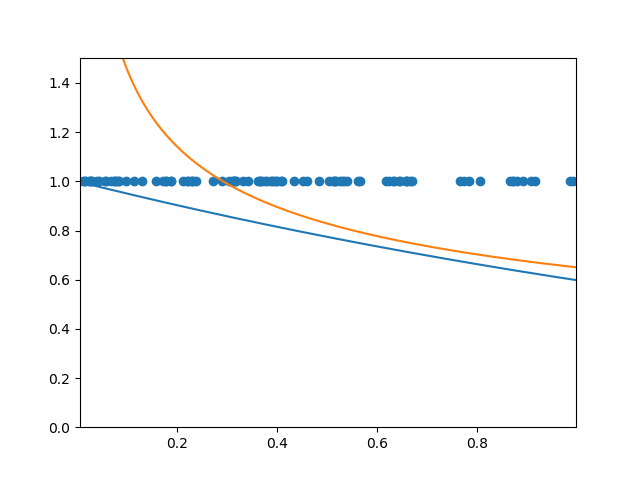
\includegraphics[scale=0.9]{graph.png}
\ \\

A curva azul representa $f(x)$. A curva laranja representa $g(x)$ e os pontos sobre a reta $y = 1$ são pontos aleatórios com distribuição $g(x)$. Como vemos, a área de $f(x)$ é maior próxima à zero, onde os pontos se concentram. Os poucos pontos próximos de $1$ são pontos "inúteis", pois, se caem longe de onde a área é grande, tudo o que eles fazem é aumentar a variância, dando a mesma informação sobre $f$ que um ponto que cai mais próximo de onde a área é grande.\\

\subsection{Escolha da $g(x)$}
\ \\

A $g(x)$ escolhida para esse método foi a função \textit{beta}, facilmente encontrada em bibliotecas como NumPy, SciPy, na forma de \textit{beta.pdf$(x,\ \alpha ,\ \beta)$}. Além da fácil utilização dessa função e de sua distribuição aleatória, ela é altamente manipulável pelos seus parâmetros $\alpha$ e $\beta$.\\
Quanto à escolha desses parâmetros, foram escolhidos "à olho". Isso é: baseado em como os pontos com distribuição \textit{beta} se distribuiam, e pela forma de \textit{beta}, intuí que bons resultados seriam obtidos com $\alpha = 0.65$ e $\beta = 1$. (Para $\beta=1$ e $0\leq \alpha <1$, a função se comporta como uma exponencial decrescente).\\

\subsection{Escolha do $n$}
\ \\

O algorítimo para a escolha do $n$ foi o mesmo que o do método \textit{Crud}. Afinal, $\frac{f(x)}{g(x)}=h(x)$, para o qual a média obtida será enviesada, mas ainda assim, se comporta como uma média.
\ \\

*RESULTADOS OBTIDOS:
Tempo de computação para $\epsilon \leq 1\%$: entre $3$ e $3.5$ segundos aproximadamente. \\
$n = 7776$ para a maior parte dos casos. \\
Erro estimado: em torno de $0.46\%$.\\
Variância amostral: em torno de $0.045$. (CALCULADO COM $95\%$ DE CONFIANÇA).\\
Integral calculada: $0.7832315934372269$ (resultados variam).\\
\ \\

Vemos que para um $n$ bem menor, obtivemos um erro bem razoável, menor do que o do método \textit{Hit-or-Miss}, mesmo com um $n$ tão menor, além de uma variância $4$ vezes menor do que a do método \textit{Crud} (vide algorítimo). A grande contrapartida de minha implementação é o tempo de computação. Eu não havia mencionado anteriormente, mas o tempo de computação, para um $n$ $10$ vezes maior é muito maior. Mais do que o dobro. Isso significa que, com minha implementação, esse método não calcula bem a integral para erros muito pequenos.\\
\ \\
Segue uma referência direta à saída do programa, comparando o Método \textit{Crud} com \textit{Importance Sampling}, para um mesmo $n$:\\
\ \\

\noindent $->$ N =  46656\\
\ $->$

\noindent $->$ Gama crud =  0.7840272530777541 x Gama IS =  0.7814250367731104\\
$->$ Var. crud =  0.16429653139693903 x Var. IS =  0.045368283893651815\\
\ \\

O \textit{Importance Sampling} é notavelmente mais preciso para um $n$ comum.

\subsubsection{Variância}
\ \\

Como a escolha do $n$ depende da minha variância, é importante discuti-la. Para esse método, o cálculo da variância é diferente do cálculo normal de uma variância.
A sua estimativa pode ser calculada de acordo com a apresentada em \href{https://statweb.stanford.edu/~owen/mc/Ch-var-is.pdf}{https://statweb.stanford.edu/~owen/mc/Ch-var-is.pdf}:
$$S^2 = \frac{1}{n}\sum_{i=1}^{n}\left(\frac{f(x_i)}{g(x_i)}-\hat{\gamma}\right)^2$$
onde $\hat{\gamma}$ é pré-fixado para o $n$. Esse cálculo resulta em uma variância amostral muito menor do que a do método \textit{Crud}, pelas propriedades explicadas anteriormente sobre esse método.
\ \\


\section{Método \textit{Control Variate}}
\ \\

Esse método também tem como objetivo principal diminuir a variância. Ele consiste em definir uma função $\phi(x)$, a qual seja muito semelhante em crescimento, posição, ou seja, o gráfico, da $f(x)$, além dela ser facilmente integrável de alguma forma (é um método especialmente útil se não sabemos integrar $f(x)$ de nenhuma forma. A idéia é que se soubermos integrar $\phi(x)$, podemos analizar a covariância que ela possui com a $f(x)$ e calcular $\hat{\gamma}$ em função dessa covariância. O que entendo desse método, de forma pouco rebuscada, é que ele aproxima a integral de $f(x)$ da intergal de $\phi(x)$ pelo quanto elas estão relacionadas. Quanto mais correlacionadas, melhor será a aproximação da integral de uma para a outra. Dessa forma, também obtemos uma variância menor.\\
\ \\

Com $f(x)$ e $\phi(x)$, calculamos dois estimadores: $\hat{\gamma_{f}}$ e $\hat{\gamma_{\phi}}$. Calculamos $\displaystyle{\int_{0}^{1}\phi(x)dx}$, além da variância amostral de $f(x)$, $Var(\hat{\gamma_f}) = S^2 = \frac{\sum_{1}^{n}(x_i - \hat{\gamma_f})^2}{n}$, com $x_i \sim U[0,1]$.\\
A covariância amostral é calculada como:
$$\displaystyle{\frac{1}{n}\sum_{i=1}^{n}(x_i - \hat{\gamma_f})(x_i -\hat{\gamma_{\phi}}})$$
Devemos definir além de tudo isso:
$$\hat{\Gamma} = \hat{\gamma_f} +c(\hat{\gamma_{\phi}-\int_{0}^{1}\phi(x)dx)}$$
onde $\displaystyle{c = -\frac{Cov(\hat{\gamma_\phi},\hat{\gamma_{f}})}{Var(\hat{\gamma_{f}})}}$ é um coeficiente ótimo, de acordo com \href{https://en.wikipedia.org/wiki/Control_variates}{Wikipedia - Control Variates}, e a variante desse $\hat{\Gamma}$:
$$\hat{\Gamma} = Var(\hat{\gamma_f}) - \frac{Cov(\hat{\gamma_f},\ \hat{\gamma_{\phi}})^2}{Var(\hat{\gamma_{\phi}})}$$

\subsection{Escolha de $\phi(x)$}
\ \\

Essa foi uma escolha fácil. Sabemos que:
$$e^u = 1 + u + \frac{u^2}{2!} +\frac{u^3}{3!} +\dots =\displaystyle{\lim_{n \to \infty} \sum_{i=0}^{n}\frac{u^i}{i!}}$$
Desse dado, tiramos, com n = 6 que:
$$\phi(x) =\cos(\beta x)\left( 1 + (-\alpha x) + \frac{(-\alpha x)^2}{2!} +\frac{(-\alpha x)^3}{3!} +\dots \right)=\cos(\beta x) \sum_{i=0}^{6}\frac{(-\alpha x)^i}{i!}$$
é uma curva aproximada de $f(x)$ no intervalo desejado e fácil de calcular a integral.\\
\ \\

No gráfico abaixo, podemos ver as duas curvas comparadas:\\
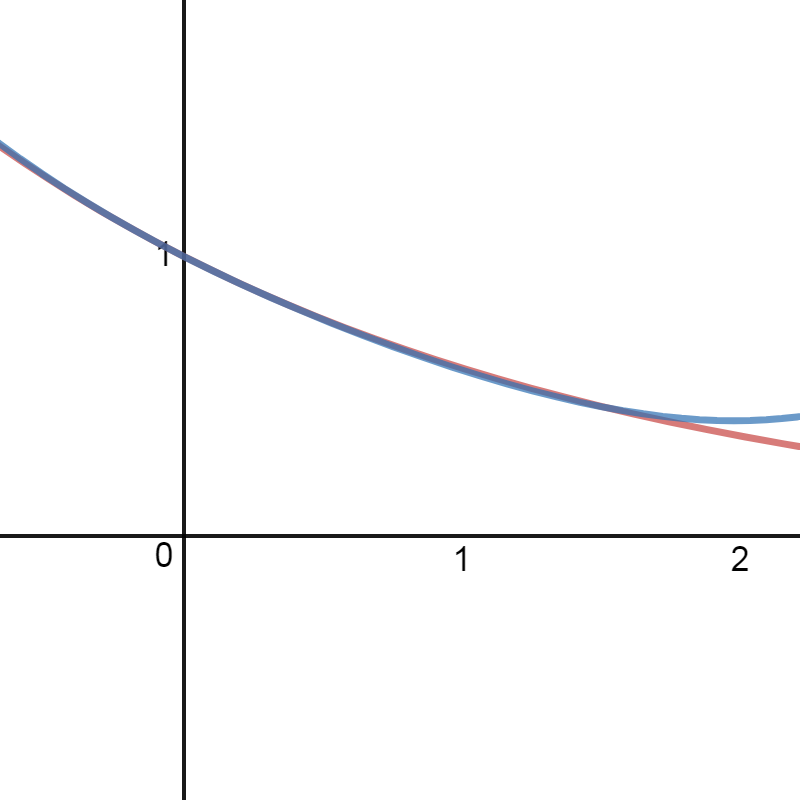
\includegraphics[scale=0.4]{desmos-graph.png}\\
Note que $f(x)$ é a curva vermelha e $\phi(x)$ a curva azul.

\subsection{Escolha do $n$}
\ \\

A escolha do $n$ se deu como todas as anteriores, notando-se que os cálculos acima, todos, devem ser feitos novamente em cada etapa. Porém, para além da complicação da implementação, os resultados são muito bons:\\
\ \\

\noindent Tempo de computação para $\epsilon \leq 1\%$: entre $1.9$ e $2$ segundos aproximadamente. \\
$n = 7776$ para a maior parte dos casos. \\
Erro estimado: em torno de $0.76\%$.\\
Variância amostral: em torno de $0.12$.\\
Integral calculada: $0.7787033368873665$ (resultados variam).\\
\ \\

Os resultados obtidos são agradáveis. Vemos que obtemos uma variância menor, para um $n$ menor, não tão boa quanto a do método \textit{Importance Sampling}, porém razoável, e um erro desejado. Além disso, o tempo de computação é melhor do que o do \textit{Importance Sampling}, o queno torna um método vantajoso. Em alguns experiomentos, pude verificar que para um $n$ maior a variância desse método se torna ainda menor. Se compararmos com o mesmo $n$ do método \textit{Crud}, veriamos uma grande melhoria. Esses vários fatores me levam a crer, que ao menos para a curva $f(x)$ que utilizamos, esse último método é o mais equilibrado em termos de eficiência e resultado.

\end{document}

%Useful info: \\
%\href{https://web.northeastern.edu/afeiguin/phys5870/phys5870/node71.html}{https://web.northeastern.edu/afeiguin/phys5870/phys5870/node71.html}